\documentclass{ctexart}
\usepackage{amsmath}
\usepackage{float}

\begin{document}
	\section{系统软件}
	\subsection{source.list}
		\indent deb http://mirrors.163.com/ubuntu/ bionic main restricted universe multiverse	\\
		\indent deb http://mirrors.163.com/ubuntu/ bionic-security main restricted universe multiverse	\\
		\indent deb http://mirrors.163.com/ubuntu/ bionic-updates main restricted universe multiverse	\\
		\indent deb http://mirrors.163.com/ubuntu/ bionic-proposed main restricted universe multiverse	\\
		\indent deb http://mirrors.163.com/ubuntu/ bionic-backports main restricted universe multiverse	\\
		\indent deb-src http://mirrors.163.com/ubuntu/ bionic main restricted universe multiverse	\\
		\indent deb-src http://mirrors.163.com/ubuntu/ bionic-security main restricted universe multiverse	\\
		\indent deb-src http://mirrors.163.com/ubuntu/ bionic-updates main restricted universe multiverse	\\
		\indent deb-src http://mirrors.163.com/ubuntu/ bionic-proposed main restricted universe multiverse	\\
		\indent deb-src http://mirrors.163.com/ubuntu/ bionic-backports main restricted universe multiverse	\\
		\indent deb http://archive.canonical.com/ bionic partner	\\
		
	\subsection{nvidia驱动}
		\noindent 查看适合的驱动
		\indent ubuntu-drivers devices	\\
		\begin{figure}[H]
			\centering
			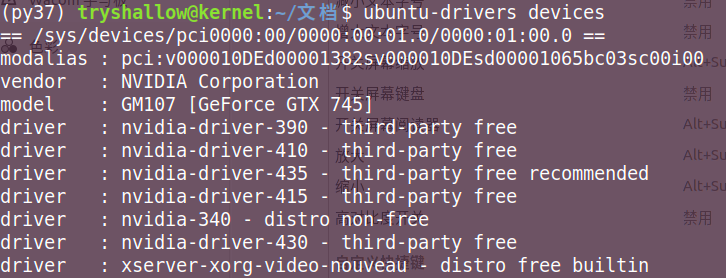
\includegraphics[width=0.7\linewidth]{asserts/ubuntu-drivers}
			\caption{ubuntu-drivers devices}
			\label{fig:ubuntu-drivers}
		\end{figure}
		\noindent 添加软件仓库	\\
		\indent sudo add-apt-repository ppa:graphics-drivers/ppa	\\
		\indent sudo update	\\
		\noindent 禁用nouveau 	\\
		\indent sudo vim /etc/modprobe.d/blacklist-nouveau.conf	\\
		\indent 在文件末尾插入:	\\
		\indent \indent blacklist nouveau	\\
		\indent \indent options nouveau modeset=0	\\
		\indent 重启,lsmod | grep nouveau 若无输出则禁用成功
		\noindent 安装nvidia	\\
		\indent sudo apt install nvidia-driver-435 \\
		\indent nvidia-smi 可查看nvidia显卡的运行状态	\\
		\begin{figure}[H]
			\centering
			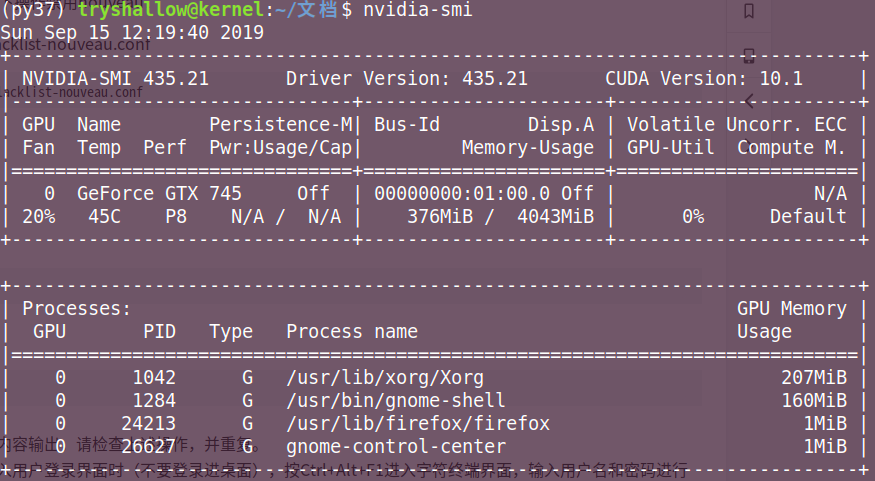
\includegraphics[width=0.7\linewidth]{asserts/nvidia-smi}
			\caption{nvidia-smi}
			\label{fig:nvidia-smi}
		\end{figure}
		
	\subsection{flashplayer安装}
		\indent sudo add-apt-repository ``deb http://archive.canonical.com/\$(lsb\_release -sc) partner''\\
		\indent sudo apt update	\\
		\indent sudo apt install adobe-flashplugin browser-plugin-freshplayer-pepperflash	\\

	\section{Python}
	\subsection{Anaconda}
	\subsubsection{.condarc}
		\noindent channels:	\\
		\indent - https://mirrors.tuna.tsinghua.edu.cn/anaconda/cloud/menpo/	\\
		\indent - https://mirrors.tuna.tsinghua.edu.cn/anaconda/cloud/bioconda/	\\
		\indent - https://mirrors.tuna.tsinghua.edu.cn/anaconda/cloud/msys2/	\\
		\indent - https://mirrors.tuna.tsinghua.edu.cn/anaconda/cloud/peterjc123/	\\
		\indent - https://mirrors.tuna.tsinghua.edu.cn/anaconda/cloud/pytorch/	\\
		\indent - https://mirrors.tuna.tsinghua.edu.cn/anaconda/cloud/conda-forge/	\\
		\indent - https://mirrors.tuna.tsinghua.edu.cn/anaconda/pkgs/main/	\\
		\indent - https://mirrors.tuna.tsinghua.edu.cn/anaconda/pkgs/free/	\\
		- defaults	\\
		\indent show\_channel\_urls: true	\\
		\indent auto\_activate\_base: false	\\
	\subsubsection{pytorch}
		conda install pytorch torchvision cudatoolkit=8.0 -c pytorch
\end{document}